\documentclass[svgnames,a4paper,final,notitlepage,10pt]{article}
\usepackage{pgfplotstable}
\usepackage{xcolor}
\definecolor{light-gray}{gray}{0.55}
\newcommand{\cbest}[1]{\textbf{#1}}
\newcommand{\notbest}[1]{\textcolor{light-gray}{#1}}
\usepackage[english]{babel}
\usepackage[utf8]{inputenc}
\usepackage[T1]{fontenc}
\usepackage{booktabs}
\usepackage[hmargin=1.2cm,vmargin=2cm]{geometry}
\usepackage{graphicx}
\usepackage{hyperref}
\usepackage{caption}
\captionsetup{format=hang,font=small}
\usepackage{subcaption}
\begin{document}

\section*{t-SNE}

\begin{figure}[htpb]
	\centering
	\includegraphics[width=\columnwidth]{tsne}
	\caption[2D projection of European venues by t-SNE]{Using code from
	\cite{}, we compute the 2D embeding of 23086 venues from 10 cities in
Europe. By taking into account all the 31 features but the category of each
venue, the method is able to roughly group venues of the same kind: Education
on the right, Nightlife on the bottom left, Professional on the bottom right
or Recreation on the top. This motivate the use of Euclidean distance in this
reduced space to measure venues similarity.\label{fig:tsne}}
\end{figure}
\clearpage

\section*{Check-in time during the day with updated data}
\begin{figure}[htpb]
	\centering
	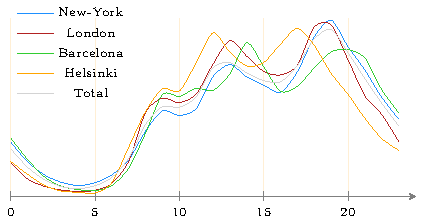
\includegraphics[width=\columnwidth]{daily_checkin}
	\caption[Pattern of check-in during the day]{Generally, the activity
		is at its lowest around 5 am and during the day, there are
		three peaks: one when people go to work in the morning, one in
		the middle of the day and the last one at the end of the
		evening. Yet, depending of the city, these peaks do not happen
		at the same time, nor with the same intensity. Therefore,
		instead of working directly the raw values of features, we use
		the number of standard deviation or \emph{z-score}.
		\label{fig:daily_checkin}}
\end{figure}

New York, the city that never sleeps, is indeed more active during the night.
\clearpage

\section*{Venues density and neighborhood radius}
\begin{figure}[h]
    \begin{subfigure}[b]{0.32\columnwidth}
        \centering
        \includegraphics[width=\textwidth]{paris_new_density_50.pdf}
    \end{subfigure}
    \begin{subfigure}[b]{0.32\columnwidth}
        \centering
	\includegraphics[width=\textwidth]{paris_new_density_160.pdf}
    \end{subfigure}
    \begin{subfigure}[b]{0.32\columnwidth}
        \centering
	\includegraphics[width=\textwidth]{paris_new_density_350.pdf}
    \end{subfigure}
\caption[Venue density in Paris]{Estimated density of 3192 venues in Paris by a
	Gaussian kernel. On the left the bandwidth is 50 meters and it looks
too small, venues are isolated, in the middle, $h=160$ because it is the maximum
likelohood estimation. On the right, $h=350$ corresponds to human definition
of neighborhood size.\label{fig:density_paris}}
\end{figure}
\clearpage

\section*{Evaluating ground metric}
\begin{table}[ht]
	\footnotesize
    \centering
\setlength{\tabcolsep}{3pt}
\begin{tabular}{llccc|ccc|ccc|ccc|ccc|ccc}
\toprule
Source & Target & \multicolumn{3}{c}{Euclidean} & \multicolumn{3}{c}{Diagonal} & \multicolumn{3}{c}{ITML} & \multicolumn{3}{c}{GB-LMNN} &
\multicolumn{3}{c}{2D t-SNE} & \multicolumn{3}{c}{Random} \\
\midrule
Berlin & San Francisco & \notbest{00} & \notbest{00} & 08 & \notbest{00} & 12 & \notbest{08} & \notbest{00} & \notbest{00} & 10 & \notbest{00} & \cbest{19} & \notbest{17} & \notbest{00} & \notbest{00} & 08 & \notbest{00} & \notbest{04} & 07 \\
Chicago & Rome & \notbest{22} & 23 & \notbest{19} & \cbest{27} & \notbest{22} & \notbest{20} & \notbest{16} & \notbest{16} & 19 & \notbest{16} & 24 & \notbest{22} & \notbest{22} & 23 & \notbest{19} & \notbest{05} & \notbest{11} & 13 \\
Helsinki & London & \cbest{36} & \notbest{20} & \notbest{16} & 27 & \notbest{15} & \notbest{23} & \notbest{18} & 25 & \notbest{14} & 27 & \notbest{25} & \notbest{19} & \cbest{36} & \notbest{20} & \notbest{16} & 18 & \notbest{15} & \notbest{14} \\
London & Helsinki & \notbest{28} & 29 & \notbest{25} & \notbest{24} & 29 & \notbest{25} & \notbest{24} & \notbest{20} & 26 & 34 & \notbest{29} & \notbest{29} & \notbest{28} & 29 & \notbest{25} & \cbest{38} & \notbest{30} & \notbest{22} \\
Moscow & Paris & \notbest{15} & \notbest{32} & \cbest{39} & \notbest{13} & \notbest{26} & 36 & \notbest{08} & \notbest{17} & 26 & \notbest{08} & \notbest{19} & 30 & \notbest{15} & \notbest{32} & \cbest{39} & \notbest{08} & \notbest{15} & 25 \\
New York & St. Louis & \notbest{06} & \notbest{08} & 09 & \notbest{04} & 08 & \notbest{08} & \cbest{12} & \notbest{12} & \notbest{09} & \notbest{10} & 11 & \notbest{09} & \notbest{06} & \notbest{08} & 09 & \notbest{04} & 06 & \notbest{05} \\
Paris & Moscow & \notbest{03} & \notbest{12} & 23 & \notbest{05} & \notbest{13} & \cbest{26} & \notbest{03} & \notbest{10} & 15 & \notbest{04} & \notbest{13} & 25 & \notbest{03} & \notbest{12} & 23 & \notbest{03} & \notbest{10} & 20 \\
Prague & Helsinki & \notbest{22} & \cbest{36} & \notbest{25} & \notbest{22} & 32 & \notbest{23} & \notbest{11} & 32 & \notbest{31} & \notbest{33} & \cbest{36} & \notbest{28} & \notbest{22} & \cbest{36} & \notbest{25} & \notbest{00} & \notbest{12} & 18 \\
Rome & Chicago & \notbest{05} & \notbest{13} & 25 & \notbest{05} & \notbest{16} & \cbest{28} & \notbest{00} & \notbest{06} & 26 & \notbest{05} & \notbest{06} & 17 & \notbest{05} & \notbest{13} & 25 & \notbest{05} & \notbest{06} & 22 \\
San Francisco & Berlin & \notbest{12} & \cbest{32} & \notbest{20} & \notbest{06} & 23 & \notbest{15} & \notbest{06} & \notbest{18} & 19 & \notbest{23} & 30 & \notbest{21} & \notbest{12} & \cbest{32} & \notbest{20} & \notbest{06} & \notbest{11} & 13 \\
Seattle & Washington & \notbest{09} & \notbest{05} & 12 & \notbest{18} & \notbest{18} & 21 & \notbest{09} & \notbest{14} & 18 & \cbest{35} & \notbest{27} & \notbest{30} & \notbest{09} & \notbest{05} & 12 & \notbest{09} & 18 & \notbest{09} \\
St. Louis & New York & \notbest{00} & \notbest{05} & 12 & \notbest{06} & \notbest{05} & \cbest{16} & \notbest{06} & \notbest{10} & \cbest{16} & \notbest{06} & \notbest{05} & 12 & \notbest{00} & \notbest{05} & 12 & \notbest{00} & 05 & \notbest{05} \\
Washington & Seattle & \notbest{04} & \notbest{03} & 07 & \notbest{00} & \cbest{14} & \notbest{10} & \notbest{04} & \notbest{02} & 08 & 12 & \notbest{11} & \notbest{10} & \notbest{04} & \notbest{03} & 07 & \notbest{04} & \notbest{06} & 07 \\
\midrule
\multicolumn{2}{c}{Winner} & \multicolumn{3}{c}{4} & \multicolumn{3}{c}{5} &
\multicolumn{3}{c}{2} & \multicolumn{3}{c}{3} &
\multicolumn{3}{c}{4} & \multicolumn{3}{c}{1}\\
\bottomrule
\end{tabular}
\caption[Metric score for brand task]{1000 times F1 score of McDonald's at level 15, 50
and 200. Cities cannot be compared because they do not have the size nor same
proportion of McDonald's.\label{tab:metric_brand}}
\end{table}

\begin{table}[ht]
	\footnotesize
	\centering
	\setlength{\tabcolsep}{3pt}
	\pgfplotstabletypeset[col sep=&,row sep=\\,fixed zerofill,precision=3,
	column type=c, skip 0.,
	columns/Source/.style={string type,column type=l},
	columns/Target/.style={string type,column type=l},
	mbest/.style={postproc cell content/.style={@cell content=\cbest{\pgfmathprintnumber[assume math mode=true,fixed zerofill,precision=3,skip 0.]{##1}}}},
	every row 0 column 4/.style=mbest,
	every row 2 column 4/.style=mbest,
	every row 6 column 4/.style=mbest,
	every row 1 column 2/.style=mbest,
	every row 3 column 2/.style=mbest,
	every row 4 column 2/.style=mbest,
	every row 5 column 2/.style=mbest,
	every head row/.style={before row=\toprule,after row=\midrule},
every last row/.style={after row=\bottomrule}]{%
	Source        & Target    & Euclidean & ITML   & GB-LMNN & 2D t-SNE & Random \\
	Prague        & Helsinki  & 0.6028    & 0.5805 & 0.6078  & 0.5906   & 0.5376 \\
	Paris         & Moscow    & 0.2843    & 0.2541 & 0.2326  & 0.1940   & 0.1340 \\
	Helsinki      & London    & 0.2536    & 0.2281 & 0.2575  & 0.2306   & 0.1563 \\
	Washington    & Seattle   & 0.3619    & 0.3251 & 0.3553  & 0.3371   & 0.2264 \\
	New York      & St. Louis & 0.5008    & 0.4684 & 0.4977  & 0.4758   & 0.3750 \\
	San Francisco & Berlin    & 0.3757    & 0.3413 & 0.3739  & 0.3506   & 0.2457 \\
	Rome          & Chicago   & 0.2219    & 0.1866 & 0.2239  & 0.2192   & 0.1400 \\
}
\caption[Metric scores for category task]{Average NDCG of each measure for
	various pair of cities. The last column shows the score obtained by returning
venues in a random order.\label{tab:metric_type}}
\end{table}

\clearpage

\section*{Measure comparison}
\begin{table}[ht]
    \centering
\begin{tabular}{lccccc}
\toprule
              & Cluster  & EMD      & EMD-LMNN & JSD      & 80\%-EMD\\% & Average \\
\midrule
Barcelona     & 0.083064 & 0.078173 & \cbest{0.084204} & 0.042414 & 0.078244\\% & \textit{0.073220} \\
New York      & 0.059200 & \cbest{0.059385} & 0.059023 & 0.057180 & 0.053495\\% & \textit{0.057656} \\
Paris         & 0.061438 & \cbest{0.091178} & 0.078614 & 0.045136 & 0.061940\\% & \textit{0.067661} \\
Rome          & 0.024313 & \cbest{0.042352} & 0.039936 & 0.021156 & 0.029746\\% & \textit{0.031501} \\
San Francisco & \cbest{0.045977} & 0.045031 & 0.040164 & 0.033829 & 0.044497\\% & \textit{0.041899} \\
Washington    & \cbest{0.043694} & 0.034762 & 0.038164 & 0.033211 & 0.038829\\% & \textit{0.037732} \\
Average       & \textit{0.052947} & \textit{\cbest{0.058480}} & \textit{0.056684} & \textit{0.038821} & \textit{0.051125}\\% & \textit{0.051612} \\
\bottomrule
\end{tabular}
\caption[Average score of each metric]{Average score of each metric when query
        are issued from the city on the left. The best metric in each city is
        \cbest{highlighted} and the last row is the average score over all
        cities.\label{tab:cmp_metric}}
\end{table}

Those figures are probably not very interesting...
\begin{figure}[h]
    \begin{subfigure}[b]{0.3\textwidth}
        \centering
        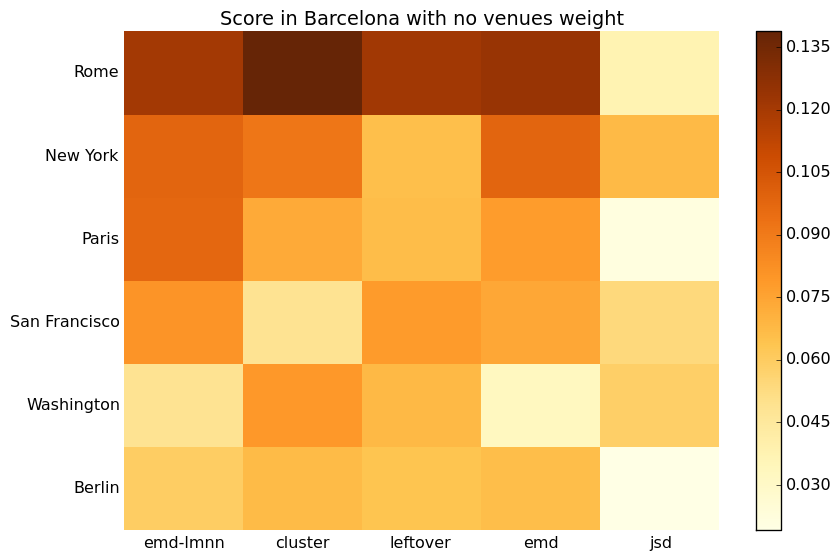
\includegraphics[width=\linewidth]{metrics_from_barcelona.png}
    \end{subfigure}~
    \begin{subfigure}[b]{0.3\textwidth}
        \centering
	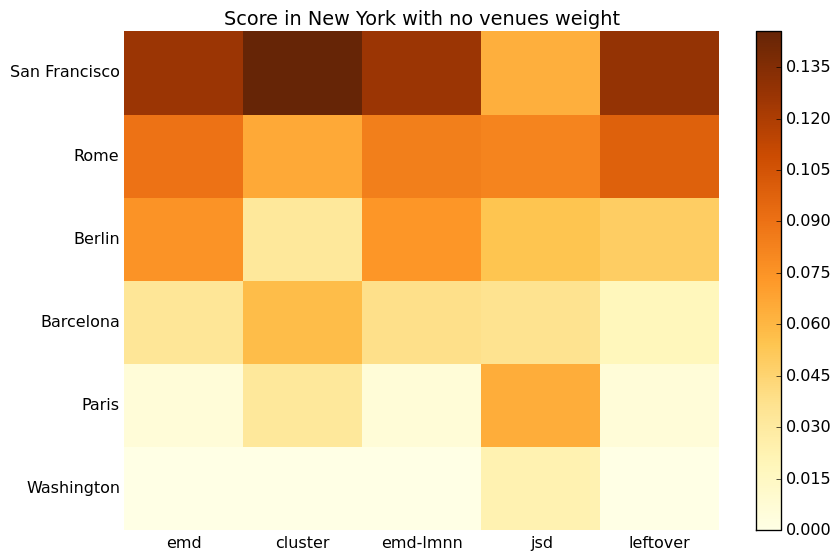
\includegraphics[width=\linewidth]{metrics_from_newyork.png}
    \end{subfigure}~
    \begin{subfigure}[b]{0.3\textwidth}
        \centering
	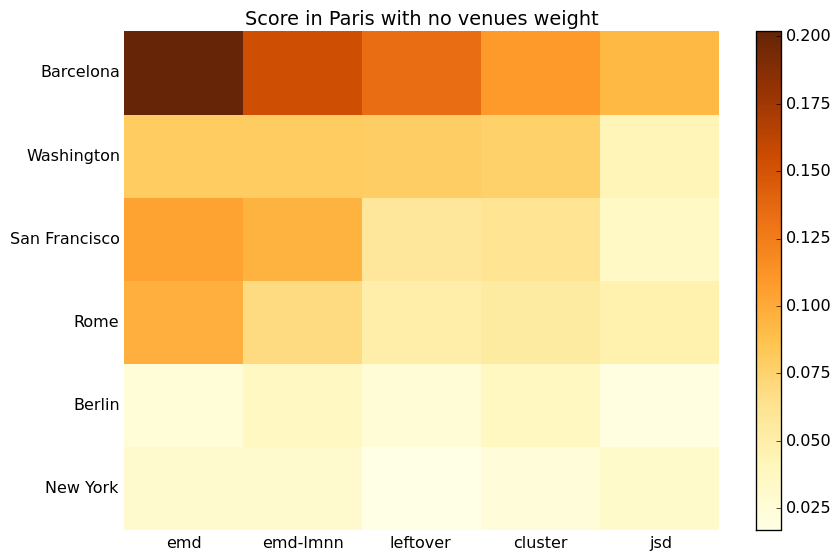
\includegraphics[width=\linewidth]{metrics_from_paris.png}
    \end{subfigure}

    \begin{subfigure}[b]{0.3\textwidth}
        \centering
	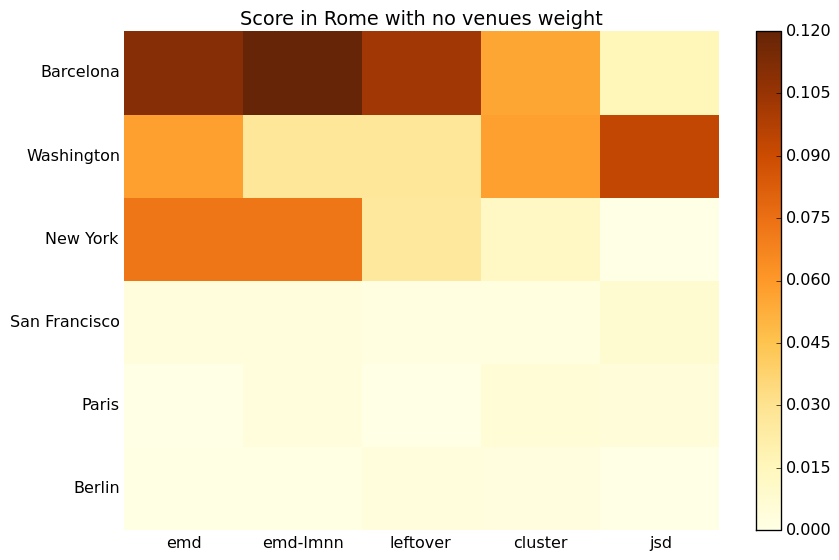
\includegraphics[width=\linewidth]{metrics_from_rome.png}
    \end{subfigure}~
    \begin{subfigure}[b]{0.3\textwidth}
        \centering
	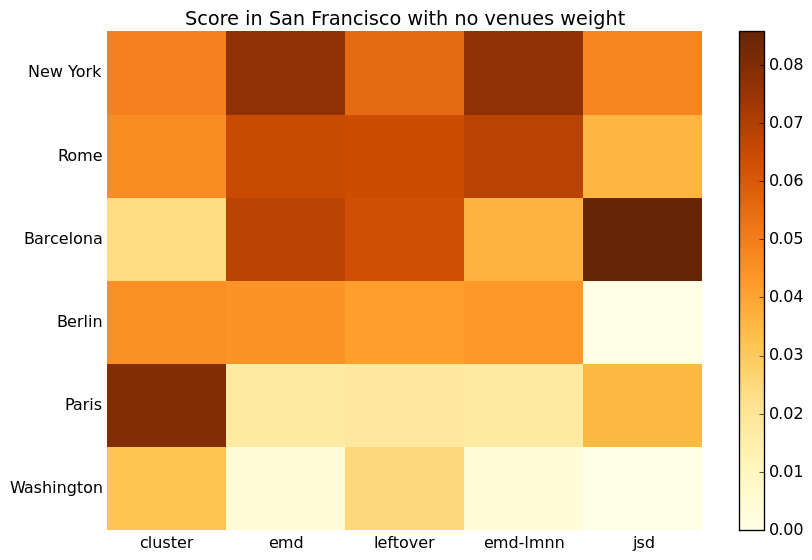
\includegraphics[width=\linewidth]{metrics_from_sanfrancisco.png}
    \end{subfigure}~
    \begin{subfigure}[b]{0.3\textwidth}
        \centering
	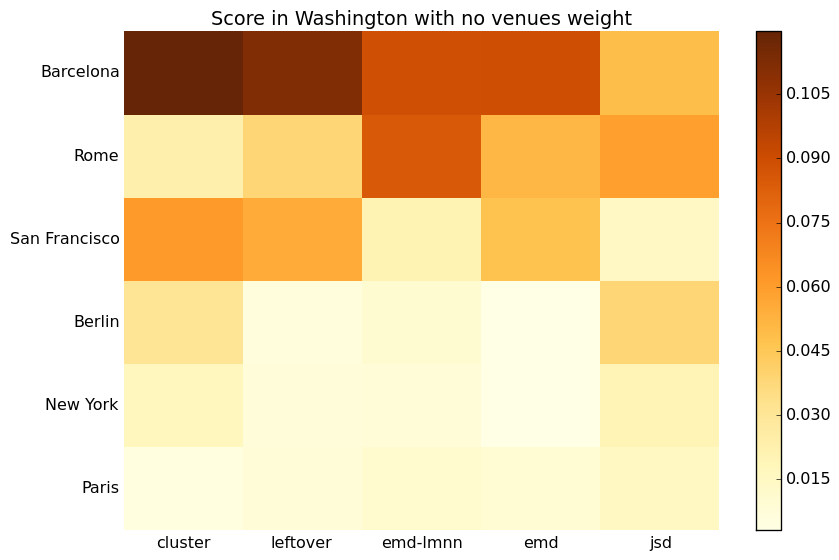
\includegraphics[width=\linewidth]{metrics_from_washington.png}
    \end{subfigure}
\end{figure}
\clearpage

\section*{One query in all cities}
Show map screenshot?
% \newgeometry{hmargin=0.2cm,vmargin=0.2cm}
\begin{center}
\begin{tabular}{llrlrlrlr}
\toprule
&\multicolumn{2}{c}{Mission, San Francisco} & \multicolumn{2}{c}{Wall Street, New York} & \multicolumn{2}{c}{Kensington, Londo}& \multicolumn{2}{c}{Soho, Londo} \\
\midrule
Rank & Cities &  Distances &            Cities &  Distances       & Cities   & Distance          & Cities &  Distances \\
\midrule
1 &     New York &        3.369 &    Los Angeles &         3.317 &          Seattle &             3.851 &                Los Angeles &         2.738 \\
2 &      Seattle &        3.380 &  San Francisco &         3.405 &          Washington &          3.944 &                     Moscow &         2.858 \\
3 &  Los Angeles &        3.386 &     Washington &         3.436 &          New York &            4.003 &                     Moscow &         2.979 \\
4 &      Seattle &        3.391 &     Washington &         3.444 &          Moscow &              4.022 &                 Washington &         3.002 \\
5 &      Seattle &        3.414 &         London &         3.468 &          New York &            4.052 &                Los Angeles &         3.029 \\
6 &   Washington &        3.424 &         London &         3.479 &          New York &            4.059 &                      Paris &         3.134 \\
7 &  Los Angeles &        3.427 &  San Francisco &         3.523 &          Chicago &             4.061 &                      Paris &         3.169 \\
8 &       London &        3.471 &        Seattle &         3.523 &          New York &            4.064 &                   Helsinki &         3.173 \\
9 &     New York &        3.477 &     Washington &         3.597 &          New York &            4.131 &                Los Angeles &         3.178 \\
10 &  Los Angeles &        3.502 &        Seattle &         3.615 &         Seattle &             4.153 &                     Houston &         3.200 \\
11 &      Chicago &        3.508 &     Washington &         3.623 &         Washington &          4.157 &                      Berlin &         3.209 \\
12 &     Chicago &        3.511 &         London &         3.627 &          Washington &          4.161 &                     Berlin &         3.219 \\
13 &     New York &        3.542 &     Washington &         3.652 &         San Francisco &       4.206 &                     Houston &         3.292 \\
14 &  Los Angeles &        3.554 &         Moscow &         3.765 &         Barcelona &           4.242 &                      Berlin &         3.292 \\
15 &      Chicago &        3.557 &        Chicago &         3.859 &         San Francisco &       4.245 &                     Houston &         3.328 \\
\midrule
% 16 &     New York &        3.564 &        Atlanta &         3.874 &       Washington &          4.246 &                     St. Louis &         3.342 \\
% 17 &      Seattle &        3.571 &        Atlanta &         3.918 &       Washington &          4.247 &                    Washington &         3.346 \\
% 18 &  Los Angeles &        3.589 &    Los Angeles &         3.988 &       San Francisco &       4.258 &                       Seattle &         3.350 \\
% 19 &   Washington &        3.598 &  San Francisco &         3.995 &       San Francisco &       4.273 &                   Los Angeles &         3.354 \\
% 20 &      Seattle &        3.615 &         Berlin &         3.996 &       Los Angeles &         4.278 &                        Berlin &         3.365 \\
% 21 &      Houston &        3.635 &      Amsterdam &         4.023 &       Paris &               4.279 &                   Los Angeles &         3.431 \\
% 22 &      Atlanta &        3.642 &  San Francisco &         4.128 &       Los Angeles &         4.299 &                       Atlanta &         3.436 \\
% 23 &       London &        3.644 &      Barcelona &         4.129 &       Seattle &             4.307 &                        Berlin &         3.444 \\
% 24 &     New York &        3.650 &        Atlanta &         4.129 &       Atlanta &             4.318 &                       Chicago &         3.459 \\
% 25 &      Atlanta &        3.653 &    Los Angeles &         4.144 &       Seattle &             4.319 &                      Helsinki &         3.482 \\
% 26 &      Chicago &        3.657 &        Houston &         4.198 &       San Francisco &       4.319 &                    Washington &         3.535 \\
% 27 &      Chicago &        3.694 &      Stockholm &         4.226 &       Seattle &             4.320 &                  Indianapolis &         3.549 \\
% 28 &   Washington &        3.735 &        Seattle &         4.227 &       Los Angeles &         4.324 &                      New York &         3.553 \\
% 29 &       Prague &        3.738 &  San Francisco &         4.248 &       Paris &               4.335 &                       Atlanta &         3.560 \\
% 30 &        Paris &        3.757 &      Amsterdam &         4.368 &       Paris &               4.340 &                    Washington &         3.574 \\
% 31 &   Washington &        3.762 &        Atlanta &         4.402 &       Berlin &              4.377 &                      New York &         3.648 \\
% 32 &   Washington &        3.774 &      Amsterdam &         4.429 &       Atlanta &             4.388 &                    Washington &         3.648 \\
% 33 &     Helsinki &        3.803 &        Seattle &         4.497 &       Barcelona &           4.398 &                       Houston &         3.653 \\
% 34 &      Atlanta &        3.823 &         Berlin &         4.539 &       Berlin &              4.418 &                     Barcelona &         3.654 \\
% 35 &    Barcelona &        3.829 &      Barcelona &         4.547 &       Moscow &              4.420 &                      New York &         3.666 \\
% 36 &      Atlanta &        3.842 &      Stockholm &         4.563 &       Los Angeles &         4.421 &                         Paris &         3.677 \\
% 37 &      Houston &        3.882 &      Barcelona &         4.582 &       Los Angeles &         4.439 &                 San Francisco &         3.680 \\
% 38 &     Helsinki &        3.895 &         Berlin &         4.607 &       Houston &             4.442 &                         Paris &         3.692 \\
% 39 &       Moscow &        3.902 &   Indianapolis &         4.639 &       Atlanta &             4.458 &                        Prague &         3.717 \\
% 40 &    St. Louis &        3.914 &        Seattle &         4.644 &       Paris &               4.467 &                       Chicago &         3.719 \\
% 41 &    St. Louis &        3.921 &   Indianapolis &         4.653 &       Chicago &             4.488 &                       Chicago &         3.726 \\
% 42 &        Paris &        3.937 &          Paris &         4.737 &       Barcelona &           4.548 &                     Barcelona &         3.750 \\
% 43 &    St. Louis &        3.944 &         Berlin &         4.811 &       Moscow &              4.566 &                         Paris &         3.771 \\
% 44 &       Moscow &        3.969 &      St. Louis &         4.848 &       Chicago &             4.576 &                     Amsterdam &         3.783 \\
% 45 &    Barcelona &        3.983 &          Paris &         4.863 &       Helsinki &            4.579 &                       Houston &         3.787 \\
% 46 &      Houston &        4.007 &          Paris &         4.868 &       Moscow &              4.588 &                       Chicago &         3.794 \\
% 47 &       Berlin &        4.010 &      Barcelona &         4.872 &       Paris &               4.591 &                     Amsterdam &         3.806 \\
% 48 &        Paris &        4.014 &         Prague &         4.878 &       Atlanta &             4.596 &                 San Francisco &         3.812 \\
% 49 &        Paris &        4.023 &      Amsterdam &         4.881 &       Atlanta &             4.614 &                      New York &         3.825 \\
% 50 &    Barcelona &        4.037 &           Rome &         4.909 &       Amsterdam &           4.620 &                     St. Louis &         3.857 \\
% 51 &       Moscow &        4.039 &        Houston &         4.913 &       Moscow &              4.629 &                     Amsterdam &         3.870 \\
% 52 &       Moscow &        4.052 &          Paris &         4.950 &       Indianapolis &        4.660 &                       Chicago &         3.875 \\
% 53 &       Berlin &        4.055 &           Rome &         4.954 &       Barcelona &           4.679 &                       Atlanta &         3.879 \\
% 54 &    Stockholm &        4.091 &         Berlin &         4.993 &       Helsinki &            4.681 &                          Rome &         3.925 \\
% 55 &       Berlin &        4.092 &        Houston &         4.995 &       Amsterdam &           4.691 &                      New York &         3.934 \\
% 56 &       Berlin &        4.092 &      St. Louis &         5.007 &       Rome &                4.694 &                  Indianapolis &         3.946 \\
% 57 &      Atlanta &        4.101 &        Atlanta &         5.063 &       Stockholm &           4.695 &                       Seattle &         3.951 \\
% 58 &       Berlin &        4.111 &       Helsinki &         5.104 &       Houston &             4.700 &                 San Francisco &         3.997 \\
% 59 &      Houston &        4.114 &      St. Louis &         5.159 &       St. Louis &           4.705 &                 San Francisco &         4.003 \\
60 &       Moscow &        4.144 &      Stockholm &         5.186 &         Berlin &              4.779 &                     Atlanta &         4.017 \\
61 &    St. Louis &        4.159 &      St. Louis &         5.210 &         St. Louis &           4.834 &                   St. Louis &         4.026 \\
62 & Indianapolis &        4.165 &      Amsterdam &         5.311 &         Prague &              4.835 &                        Rome &         4.056 \\
63 &       London &        4.178 &         Prague &         5.319 &         Barcelona &           4.859 &                     Atlanta &         4.057 \\
64 &      Houston &        4.183 &           Rome &         5.346 &         Houston &             4.887 &                   Barcelona &         4.079 \\
65 &    Amsterdam &        4.183 &       Helsinki &         5.397 &         Houston &             4.907 &                        Rome &         4.081 \\
66 &       Prague &        4.207 &           Rome &         5.696 &         Amsterdam &           4.908 &                   Amsterdam &         4.149 \\
\bottomrule
\end{tabular}
\end{center}
% \restoregeometry

The full map is at \href{http://daureg.github.io/hairy-octo-archer/world/}% 
{\url{daureg.github.io/hairy-octo-archer/world}}. Holding Shift while drawing a rectangle
zoom on the map and pressing \texttt{M}, \texttt{K}, \texttt{W} and \texttt{S} change to
the corresponding query.  Here are some quick comments:

\begin{itemize}
	\item Most the top results I looked were pretty small in my
		opinion.
	\item Larger cities are better ranked.
	\item European cities are better ranked for the London query than for
		US queries.
	\item For Mission the first results are in Williamsburg for NYC,
		Ballard for Seattle (Scandinavian neighborhood according to
		Wikipedia?) and somewhere in Hollywood for LA.
	\item For Wall Street, also Hollywood in LA (so not really financial
		district), Downtown San Francisco and close to the White House
		in Washington.
	\item For Soho/Picadilly Circus and Downtown LA and two places in
		Moscow (but I can't make any comments on that).
\end{itemize}
\clearpage

\section*{Approximation performance}
I will do the same as next page while varying number of neighbors tomorrow.

\begin{figure}[h]
    \begin{subfigure}[b]{\columnwidth}
        \centering
        \includegraphics[height=0.4\textheight]{nbox}
	\caption[Approximation ratio]{The approximate method give results
		whose distance ratio is close to 1 and generally under 1.5.
	\label{fig:distance_ratio}}
    \end{subfigure}

    \begin{subfigure}[b]{\textwidth}
        \centering
        \includegraphics[height=0.4\textheight]{time_ratio}
	\caption[Time speed-up]{If we sort queries by how much time they need
	to be completed, we see that our approximation scheme is order of
magnitude faster than brute force search.\label{fig:time_5steps}}
    \end{subfigure}
    \caption{Approximation trade off while increasing regions size.\label{fig:approx_size}}
\end{figure}
\clearpage
\end{document}
